Psittacine is a conlang set in the near future of the real world.
As they have done for millenia, humans continue to devastate the environment.
The rainforests continue shrinking and many animals are losing their habitat.
Under the threat of extinction,
parrots put their intelligence to use and create their own language,
and are using it to plot the downfall of humanity.

\begin{wrapfigure}{R}{0.46\textwidth}
    \caption{Alex performing a counting task.}
    \centering
    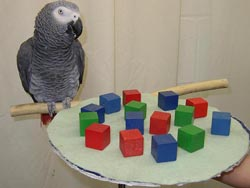
\includegraphics[scale=0.7]{alex}\label{fig:figure}
\end{wrapfigure}

Parrots are known to be some of the smartest non-human animals,
alongside great apes, dolphins, octopuses, elephants, and crows.
The possibility of parrots developing their own human-like language is not completely unreasonable.
Famously, many of them can imitate human language,
and a few
have claims to using and understanding human language.
Alex (\url{https://en.wikipedia.org/wiki/Alex_(parrot)}) was able to
perform remarkably complex tasks,
such as counting the number of objects with combinations of properties.
Alex also has been reported to be the only non-human animal to ever ask a question.

Parrots have very different physiology from humans,
but the sounds they will have in their language will be human-producible sounds.
Parrots can easily produce stops, fricatives, nasals, and a full range of vowels in a full range of phonations,
as well as many sounds humans cannot produce, such as chirps, beeps, and rapidly alternating tones.
I will only use sounds parrots and humans can both produce easily.
Since parrots don't have lips, their language will not have labial consonants or lip rounding.
(Alex reportedly had difficulty pronouncing ``paper''.)
The beak doesn't have teeth or an alveolar ridge,
but placing the tongue in approximately similar locations can make similar formant profiles.
The part of a parrot's brain responsible for cognition is the HVC,
originally purposed for processing and producing birdsong.
Since parrot language will have influence from birdsong,
it will be more reliant on tones than most human languages.

In the world of human expansion,
there are a number of different groups of parrots that
have unique interactions with humans and each other.
There are wild parrots from the rainforests who want to preserve their habitat,
and most of them want to destroy the humans.
There are feral urban parrots,
some who want to stop the humans and some who don't particularly care.
There are also domesticated parrots,
who mostly like humans (since those who don't run away).
The language has dialects that vary over the above groups, and by location.
Parrots and humans may learn each others' languages,
but have trouble producing certain sounds.

Parrots will also have their own writing system (not detailed in this book).
Some parrots may learn to use pens, but
the most natural way for parrots to write is to make scratches in bark using their beaks.
Parrots beaks have more strength and fine control than claws.
The writing system will consist mostly of short, straight strokes to reflect the medium of writing.

Parrots live all over the world, mostly in tropical areas.
Typical intelligent parrots live in natural hollows in tree canopies,
eat seeds, nuts, fruits, and occasionally bugs,
and are generally monogamous and nonterritorial.
Like humans, they are very social,
and their society could reasonably be organized similarly to that of humans.
In the story, they will develop government as they need high-level cooperation
to work against the humans.
They will also learn to use some technology.
Vocabulary and metaphors, including ones for the new technology,
will show influence from their social and dietary habits.

